%%%%%%%%%%%%%%%%%%%%%%%%%%%%%%%%%%%%%%%%%%%%%%%%%%%%%%%%%%%%%%%%
%2345678901234567890123456789012345678901234567890123456789012345678901234567890
%        1         2         3         4         5         6         7         8

\documentclass[letterpaper, 10 pt, conference]{ieeeconf}  % Comment this line out
                                                          % if you need a4paper
%\documentclass[a4paper, 10pt, conference]{ieeeconf}      % Use this line for a4
                                                          % paper

\IEEEoverridecommandlockouts                % This command is only
                                                          % needed if you want to
                                                          % use the \thanks command
\overrideIEEEmargins
% See the \addtolength command later in the file to balance the column lengths
% on the last page of the document

% The following packages can be found on http:\\www.ctan.org
\usepackage{yaacro}
\usepackage{graphicx}
\usepackage[english]{babel}
\usepackage[utf8]{inputenc}
\usepackage{multirow}
\usepackage{array}
% \usepackage{subfigure}
\usepackage{algorithm}
\usepackage{algorithmic}
% \usepackage{subfigure} %% depracated %%
\usepackage{amsmath,amssymb}
\usepackage{color}
\usepackage{booktabs}
\usepackage{microtype}
\usepackage{caption}
\usepackage{subcaption}

% \usepackage{multicol}

\graphicspath{{./figures/}}
\DeclareGraphicsExtensions{.pdf,.jpeg,.png}

\title{\LARGE \bf
Platform for Communication and Coordination of Agents using the MAVLink Protocol
}

\newcommand{\aand}{\hspace{.6cm}}

% \begin{acgroupdef}[list=acronimos]
%   \acdef{CNPq}{Conselho Nacional de Desenvolvimento Científico e Tecnológico}
%   \acdef{CAPES}{Coordenação de Aperfeiçoamento de Pessoal de Nível Superior}
%   \acdef{FAPEMIG}{Fundação de Amparo ? Pesquisa do Estado de Minas Gerais}
%   \acdef{FUCAPI}{Fundação Centro de Análise, Pesquisa e Inovação Tecnológica}
% \end{acgroupdef}

% \author{Ramon Soares de Melo
   % \thanks{Developed with the support of CNPq, CAPES and FAPEMIG.}
   %  \thanks{$^{1}$The authors are with the Computer Vision and Robotics Laboratory (VeRLab), Computer Science Department, Universidade Federal de Minas Gerais, MG, Brazil. E-mails: {\tt\small \{ramonmelo,doug,mario\}@dcc.ufmg.br}.}
% }%

\author{
    \authorblockN{Ramon Soares de Melo and Arturo César Alvarez Cea}
    \authorblockA{Universidade Federal de Minas Gerais, University of Santiago de Chile
    \\ramonmelo@dcc.ufmg.br, arturo.alvarez@usach.cl}
}

\newtheorem{definition}{Problem}[section]

\makeatletter
\newcommand{\todo}[1]{{\color{red}\textbf{{\large @TODO\@ifempty{#1}{}{: }}#1}}}
\makeatother

\begin{document}

\maketitle
\thispagestyle{empty}
\pagestyle{empty}


\newcommand{\mrs}{MRS}
\newcommand{\environment}{\ensuremath{\mathbb{R}^3}}

% Shortcut definitions

\newcommand{\set}[1]{\ensuremath{\boldsymbol{\mathcal{#1}}}}
\newcommand{\setitem}[2]{\ensuremath{#1_{#2}}}
\newcommand{\setlist}[3]{#1\ $=$\ \{\setitem{#2}{1}, \setitem{#2}{2}, ..., \setitem{#2}{#3}\}}

\newcommand{\robotset}{\set{R}} % conjunto de robôs
\newcommand{\robotsetqt}{\ensuremath{k}}
\newcommand{\robot}[1]{\setitem{r}{#1}}
\newcommand{\robotlist}{\setlist{\robotset}{r}{\robotsetqt}}

\newcommand{\obstacleset}{\set{B}} % conjunto de obstáculos
\newcommand{\obstaclesetqt}{\ensuremath{x}}
\newcommand{\obstacle}[1]{\setitem{b}{#1}}
\newcommand{\obstaclelist}{\setlist{\obstacleset}{b}{\obstaclesetqt}}

\newcommand{\objectset}{\set{O}} % conjunto de objetos
\newcommand{\objectsetqt}{\ensuremath{y}}
\newcommand{\object}[1]{\setitem{o}{#1}}
\newcommand{\objectlist}{\setlist{\objectset}{o}{\objectsetqt}}

\newcommand{\planset}{\set{P}} % plano
\newcommand{\plansetqt}{\ensuremath{q}}
\newcommand{\plan}[1]{\setitem{n}{#1}}
\newcommand{\planlist}{\setlist{\planset}{n}{\plansetqt}}

\newcommand{\robotplanset}{\set{RP}} % conjunto de planos
\newcommand{\robotplansetqt}{\ensuremath{j}}
\newcommand{\robotplan}[1]{\setitem{rp}{#1}}
\newcommand{\robotplanlist}{\setlist{\robotplanset}{rp}{\robotplansetqt}}

\newcommand{\executionplanset}{\set{EP}} % conjunto de planos
\newcommand{\executionplansetqt}{\ensuremath{h}}
\newcommand{\executionplan}[1]{\setitem{ep}{#1}}
\newcommand{\executionplanlist}{\setlist{\executionplanset}{ep}{\executionplansetqt}}
\newcommand{\executionplanname}{\emph{Execution Plan}}
\newcommand{\executionplansetnotation}{\ensuremath{\executionplanset \subset \robotplanset}}

\newcommand{\executionplanminset}{\ensuremath{\executionplanset{*}}} % conjunto com custo minimo de segmentos

\newcommand{\segmentset}{\set{S}} % conjunto de segmentos
\newcommand{\segmentsetqt}{\ensuremath{e}}
\newcommand{\segment}[1]{\setitem{s}{#1}}
\newcommand{\segmentlist}{\setlist{\segmentset}{s}{\segmentsetqt}}

\newcommand{\segmentpointset}{\ensuremath{\set{S}_p}} % conjunto de pontos de segmentação
\newcommand{\segmentpointsetqt}{\ensuremath{z}}
\newcommand{\segmentpoint}[1]{\setitem{sp}{#1}}
\newcommand{\segmentpointfirst}[1]{\ensuremath{\segmentpoint{#1}^1}}
\newcommand{\segmentpointsecond}[1]{\ensuremath{\segmentpoint{#1}^2}}

\newcommand{\segmentpointlist}{\setlist{\segmentpointset}{sp}{\segmentpointsetqt}}

\newcommand{\typeland}{ground}
\newcommand{\typeaerial}{aerial}
\newcommand{\typeset}{\set{T}} % conjunto de tipos de movimentação
\newcommand{\typelist}{\ensuremath{\typeset=\ \{}\typeland, \typeaerial\ensuremath{\}}}
\newcommand{\type}[1]{\setitem{t}{#1}}

\newcommand{\plantypestart}{initial}
\newcommand{\plantypetransition}{transition}
\newcommand{\plantypemove}{movement}
\newcommand{\plantypeset}{\set{TP}} % conjunto de tipos de plano
\newcommand{\plantypelist}{\ensuremath{\plantypeset=\ \{}\plantypestart, \plantypetransition, \plantypemove\ensuremath{\}}}
\newcommand{\plantype}[1]{\setitem{tp}{#1}}

\newcommand{\movementtypepremove}{pre-transport}
\newcommand{\movementtypemove}{transport}
\newcommand{\movementtypeset}{\set{T_m}} % conjunto de tipos de plano
\newcommand{\movementtypelist}{\ensuremath{\movementtypeset=\ \{}\movementtypepremove, \movementtypemove\ensuremath{\}}}
\newcommand{\movementtype}[1]{\setitem{tm}{#1}}

\newcommand{\tokenset}{\set{TO}}
\newcommand{\tokensetqt}{\ensuremath{u}}
\newcommand{\tokeni}[1]{\setitem{to}{#1}}
\newcommand{\token}{\emph{token}}
\newcommand{\tokenlist}{\setlist{\tokenset}{to}{\tokensetqt}}

\newcommand{\workspace2}{\ensuremath{\boldsymbol{\mathcal{W}}}} % àrea de trabalho
\newcommand{\workspacecell}{\ensuremath{\boldsymbol{\mathcal{c}}}} % àrea de trabalho

\newcommand{\allocationgraph}{\ensuremath{\mathcal{AG}}}
\newcommand{\allocationgraphcompress}{\ensuremath{\mathcal{AG}_c}}

\newcommand{\currentstate}{\ensuremath{S}}
\newcommand{\nextstate}{\ensuremath{S'}}
\newcommand{\originstate}{\ensuremath{S_o}}
\newcommand{\targetstate}{\ensuremath{S_d}}
\newcommand{\robotstate}{\ensuremath{S_r}}

\newcommand{\robotinitialstate}{\ensuremath{I}}
\newcommand{\robotinitialstatei}[1]{\ensuremath{I_{#1}}}

\newcommand{\celldimension}{\ensuremath{d}}
\newcommand{\deslocationfactor}{\ensuremath{l}}

\newcommand{\movementset}{\set{M}}
\newcommand{\movementslist}{\ensuremath{\movementset=\ \{}left, right, front, back, up, down\ensuremath{\}}}
\newcommand{\movementaction}{\ensuremath{a_i}}

% Funções

\newcommand{\utilityfunction}{\ensuremath{\Theta}}
\newcommand{\utilityplanfunction}{\ensuremath{\utilityfunction_{p}}}
\newcommand{\utilitytotalfunction}{\ensuremath{\utilityfunction_{t}}}
\newcommand{\distancefunction}{\ensuremath{\Delta}}
\newcommand{\timefunction}{\ensuremath{\Upsilon}}
\newcommand{\energyfunction}{\ensuremath{\Psi}}

% Planejamento

\newcommand{\fringe}{\set{F}}
\newcommand{\searchednodes}{\set{SN}}
\newcommand{\node}{\ensuremath{n}}
\newcommand{\nodeitem}[1]{\ensuremath{\node_{#1}}}
\newcommand{\nodeparent}{\emph{NodePai}}
\newcommand{\nodeutility}{\ensuremath{\omega}}
\newcommand{\nodedata}{\ensuremath{\{}state (\currentstate), action (\movementaction), utility (\nodeutility), agent's position (\robotstate), type (\type{i})\ensuremath{\}}}


\newcommand{\img}[4]{
  \begin{figure}[ht!]
    \centering
    \includegraphics[width=#2]{img/#1}
    \caption{#3}
    \label{fig:#4}
  \end{figure}
}


\section{INTRODUCTION}
\label{sec:introduction}

% Intro

% The use of mobile robots in many different contexts and applications has increased significantly in recent years. It is notorious the use of these autonomous systems in activities such as surveillance, search and rescue, object transportation, among others.

The use of autonomous robot systems can be seen in many scenarios, besides the industrial use, where were first employed, mainly on object manipulation and building of items in assembly lines (\cite{Rol2011}), is notorious the use of these autonomous systems in other activities like surveillance and regions recognition (\cite{Tanner2007, Sujit2013}), search and rescue (\cite{Casper2003, Murphy2004}), mapping (\cite{Tokekar2013}), detection and tracking (\cite{Grocholsky2006}), transport of objects (\cite{Michael2011, Fink2008}), among others.

All aforementioned activities can be executed both individually as well collaboratively, in this case called Multi-Robot Systems (\mrs).
The use of multiple robots presents several advantages like increased robustness and, in most cases, time reduction to accomplish a task. However, the use of such systems also brings many challenges, such as robot localization, path planning, task allocation and control.

The accomplishment of any task using a \mrs\ involves many subproblems that must be considered.
Among these problems, we can highlight the localization of the robots, path planning, coordination and the task allocation.
The localization problem is related with agent itself as well the environment where the robots are working and any other object that they interact.
The path planning problem can be addressed in many ways, in some cases to minimize the total time spent or the overall traveled distance for example.
Regarding the team coordination, that involves task allocation among the agents, as well a study of how combine the available resources to accomplish the activity respecting all possible restrictions.

% ArduPilot, MAVLink

Each agent in a \mrs\ have its own capabilities and resources, that can be shared among the other agents of the team.
These resources can be the locomotion type of the vehicle, a set of sensors, or the payload among others.
A team of agents should be able to share and explore these resources to complete satisfactorily one particular mission.

One of the platforms that has come into common use for the creation of autonomous agents is called ArduPilot (APM), whose main goal is to be an autopilot system to carry out autonomous missions, responsible for low-level control of different kinds of vehicles, such as the terrestrial ackerman model or flying with multiple rotor and fixed wing.

Similar to other platforms for autonomous control, the APM system uses the Micro Air Vehicle Communication Protocol (MAVLink) that describes a specification for data exchange between the vehicle and a base station.
It's able to transfer telemetry information such as data from sensors (GPS, barometer, magnetometer) or send missions to the agent.

Using this toolkit, a vehicle controlled by an auto pilot and having communication with a base station, can perform activities like scanning and capturing images of a particular area, carrying out autonomous missions in a consistent and easily configurable way.

% Description

The project presented here was developed during the interchange period occurred at the University of Santiago de Chile (USACH) between April and May of 2015, together with the tutor Arturo César Alvarez Cea, which has developed a base system for communication and control agents using MAVLink protocol.

% section introduction (end)

% \section{RELATED WORK}
\label{sec:related_work}

% \section{PROBLEM STATEMENT} % (fold)
\label{sec:problem_statement}









% Be an environment defined in an Euclidean space $\mathbb{R}^2$, we define by $\mathcal{W} \subset \mathbb{R}^2$ a convex polygon as the workspace in the environment.

% Let $\mathcal{R} = \{r_1, r_2, ..., r_k\}$ be a set of $k$ ground agents that only have the capacity to push objects using it's own body.
% Is defined by $\mathcal{O} = \{o_1, o_2, ..., o_n\}$ the set of $n$ objects that must be transported.
% All object $o \in \mathcal{O}$ are uniformly distributed in the workspace $\mathcal{W}$.
% Likewise, is defined the set $\mathcal{B} = \{b_1, b_2, ..., b_m\}$ of $m$ blocking objects that are immovable and will restrict the movement of the agents and the objects.

% To realize the transport phase, each object $o \in \mathcal{O}$ calculates a set of paths within the environment that the agents must accomplish to transport the object to its destination.
% These paths are broken into sub-paths if necessary, and included in the set $\mathcal{P} = \{sp_1, sp_2, ..., sp_j\}$.
% Each sub-path $sp \in \mathcal{P}$ is a set of points $p \in \mathcal{W}$, and represents a task in the context of task allocation.

% section problem_statement (end)

\section{METHODOLOGY}
\label{sec:methodology}

The main objective of this work was the creation of a base system for communication and exchange of information between autonomous agents through MAVLink protocol.
Agents must be able to share informations such as your current position, your current status (whether they are on a mission or not), what mission they are in, as well as having the ability to send missions to other agents.

The project was based on framework ROS (Robot Operating System), which provides a platform for research and development of robotic systems, possessing abstraction layers for communication, visualization and others.
As control platform, the autopilot ArduPilot had been used in two different kind vehicles, a land based (figure \ref{fig:rover}) and aerial (figure \ref{fig:quad}).
Both have global positioning sensor (GPS), altitude, and communication via radio, which can send and receive data from a base station.

\begin{figure}
        \centering
        \begin{subfigure}[b]{0.3\textwidth}
                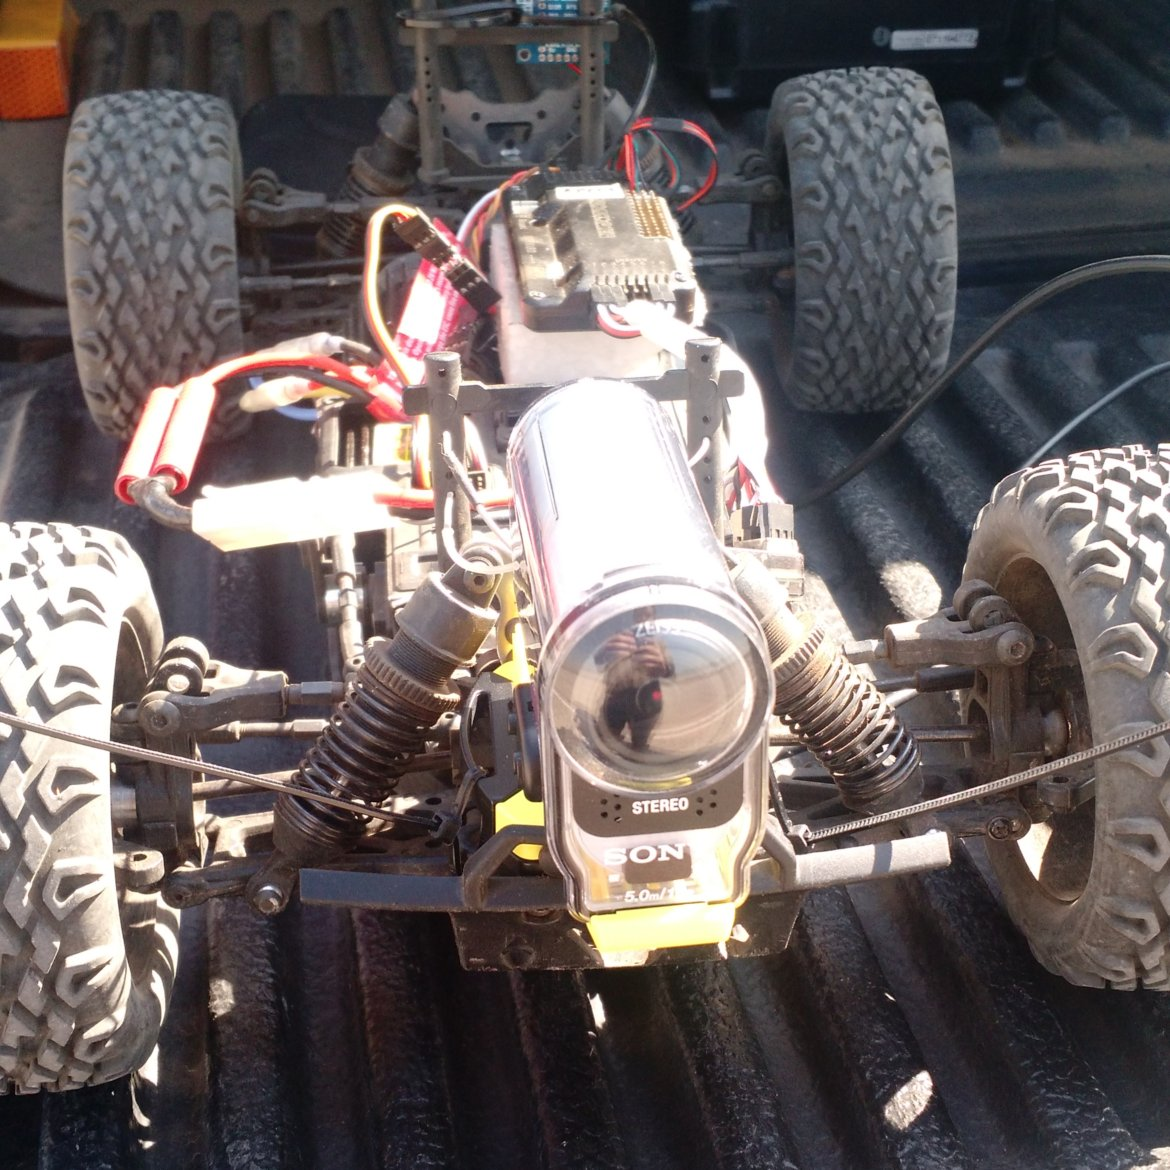
\includegraphics[width=\textwidth]{img/rover.jpg}
                \caption{Rover}
                \label{fig:rover}
        \end{subfigure}
        \quad
        \begin{subfigure}[b]{0.3\textwidth}
                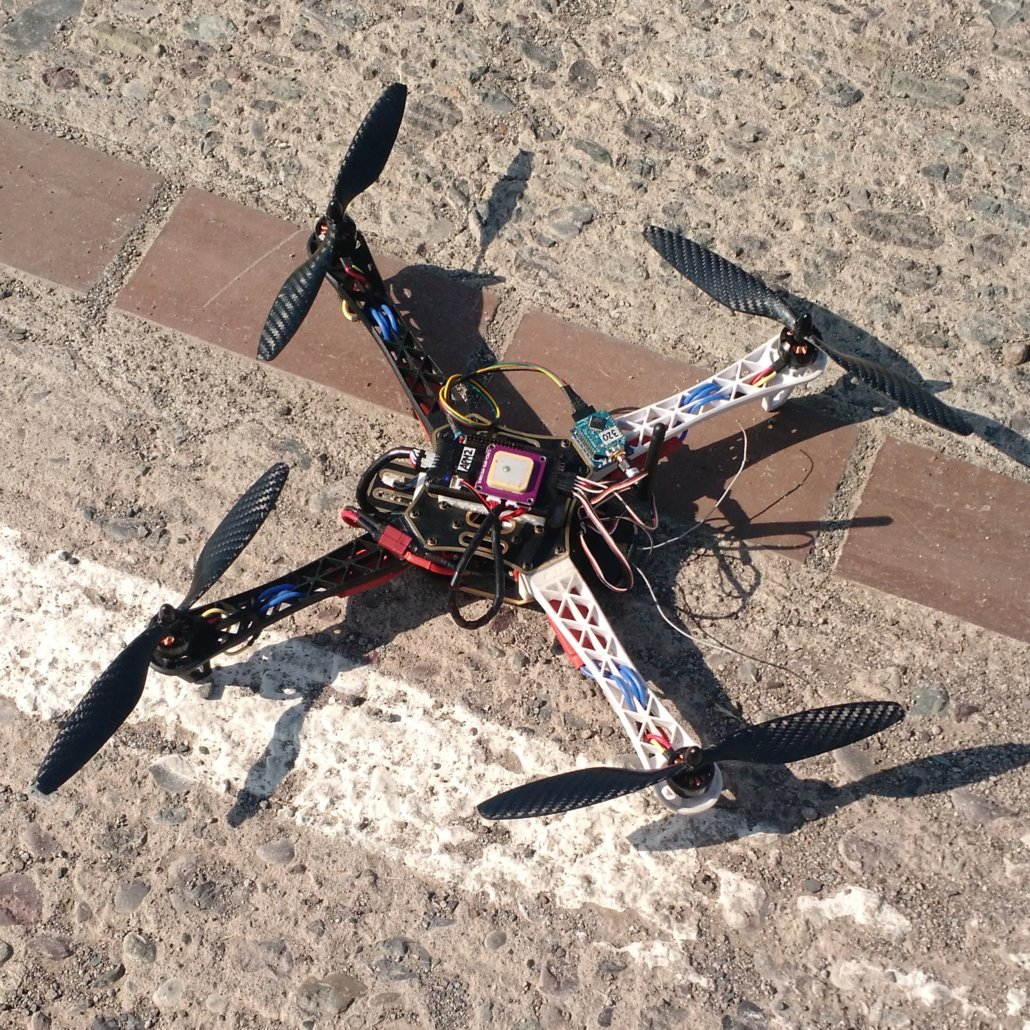
\includegraphics[width=\textwidth]{img/quad.jpg}
                \caption{Quadcopter}
                \label{fig:quad}
        \end{subfigure}
        \caption{Agents used on experiments}
        \label{fig:agents}
\end{figure}

\subsection{MAVLink Protocol} % (fold)
\label{sub:mavlink_protocol}

The MAVLink protocol was constructed to serve as common language between a ground control station and a autonomous robot.
It shows how to encode and decode data using a header-only message, describing a set of message types used to identify the message content.

A MAVLink message consists of a package with a minimum of 8 bytes and 263 bytes as maximum.
As can be seen in the figure \ref{fig:mavlink_message}, the package is divided into several slots, each one with a specific description.
The table \ref{table:mavlink_package} list and describe all slots of a MAVLink package.

\begin{figure}
  \centering
  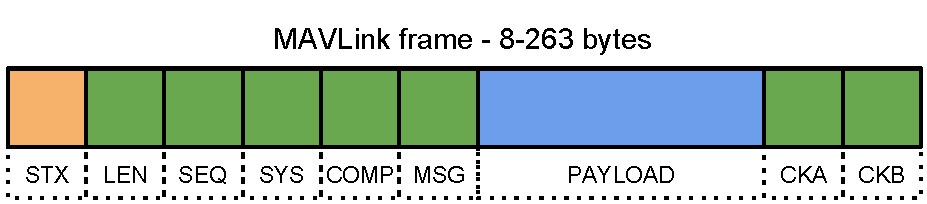
\includegraphics[width=0.9\columnwidth]{img/MAVLinkpackage.pdf}
  \caption{MAVLink Package description}
  \label{fig:mavlink_message}
\end{figure}

\begin{table}
    \begin{tabular}{|m{0.15\columnwidth}|m{0.75\columnwidth}|}
    \hline
    Slot    & Description                                                              \\ \hline
    STX     & Indicate a new package                                                   \\ \hline
    LEN     & Indicate the total length of the payload                                 \\ \hline
    SEQ     & Package sequence                                                         \\ \hline
    SYS     & ID of the sending MAV system                                             \\ \hline
    COMP    & ID of the sending component inside the MAV                               \\ \hline
    MSG     & ID of the message describing what type of message will be in the payload \\ \hline
    PAYLOAD & Data of the message                                                      \\ \hline
    CKA     & Checksum A (low byte)                                                    \\ \hline
    CKB     & Checksum B (high byte)                                                   \\ \hline
    \end{tabular}
    \caption {MAVLink Package slot description}
    \label{table:mavlink_package}
\end{table}

The protocol can handle various types of data, having support to fixed-size integer data, floats with single precision point, and array of these types.
The supported types are: \emph{char, uint8, int8, uint16, int16, uint32, int32, uint64, int64, float, double}.

The main objective of the protocol was the be fast and safety, but there are some drawbacks, as the need of extra bytes to track the messages, but it can detect the lost of packages and check the content.

% subsection mavlink_protocol (end)

\subsection{ROS Communication System} % (fold)
\label{sub:ros_communication_system}

The ROS environment was created aiming the decoupling between any part of the system, creating a system of communication that do not link directly two parts of the code.
To create this environment, two main concepts were created, the nodes and the topics.
Each node is a piece of code that executes a determined behavior, like control the velocity of the motors of a car or capture images from a camera.
Each topic is a address where the data is read and write by the nodes using the actions of subscribing and/or publishing to that topic.
This guarantee the possibility of the code run in different computers, like using a team of robots, each one with it individual computer for example.

The figure \ref{fig:ros_environment} show a representation of the ROS environment, where there are many nodes exchanging information using the topics. One important note about that type of communication is about the registration of the nodes and the initial meeting among then, that is made by the called \emph{master node}, that waits for the initialization of any node, and any request to publish or subscribe to one topic and make all the necessary connections.

\begin{figure}
  \centering
  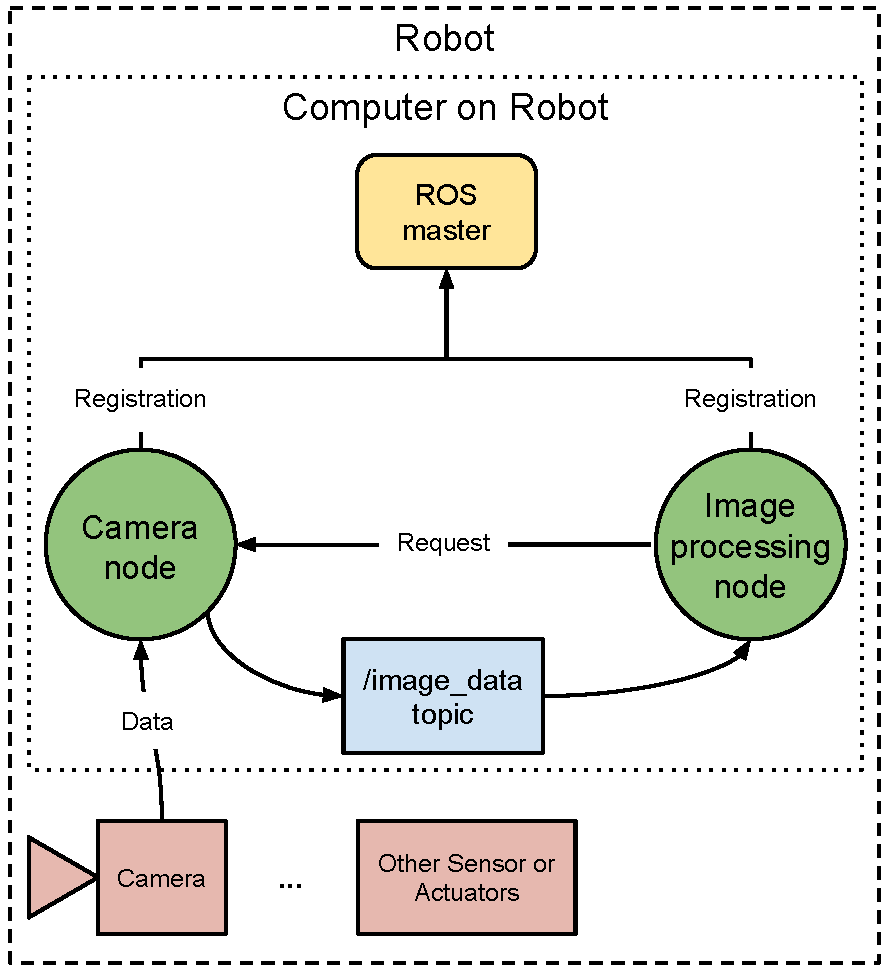
\includegraphics[width=0.9\columnwidth]{img/ros_environment.pdf}
  \caption{ROS Environment}
  \label{fig:ros_environment}
\end{figure}

% subsection ros_communication_system (end)

\subsection{Project Architecture} % (fold)
\label{sub:architecture}

In general, the architecture for controlling a robot using the ArduPilot platform is made by a base station which communicates with the agent via the MAVLink protocol, sending commands and tasks.
The onboard controller is responsible to receive and threat theses messages, making the necessary decisions to accomplish the sent objectives.
However, this strategy only guarantees the control of one agent at a time, and does not allow the exchange of information between an agent team.
The work developed here proposes an extension to this architecture in order to provide a communication and intelligence layer for agents, serving as basis for the development of more complex tasks that require the use of a set of robots.

Figure \ref{fig:architecture} shows the layout of the developed architecture, marking the addition in the context of communication in the pre-existing control layer.
The manner in which this strategy was set aims to promote transparency about the origin of the commands received by the agents, because similar to messages sent by the base station, the system developed also communicates through MAVLink commands, which makes interaction with agents direct and simple.

\begin{figure}
  \centering
  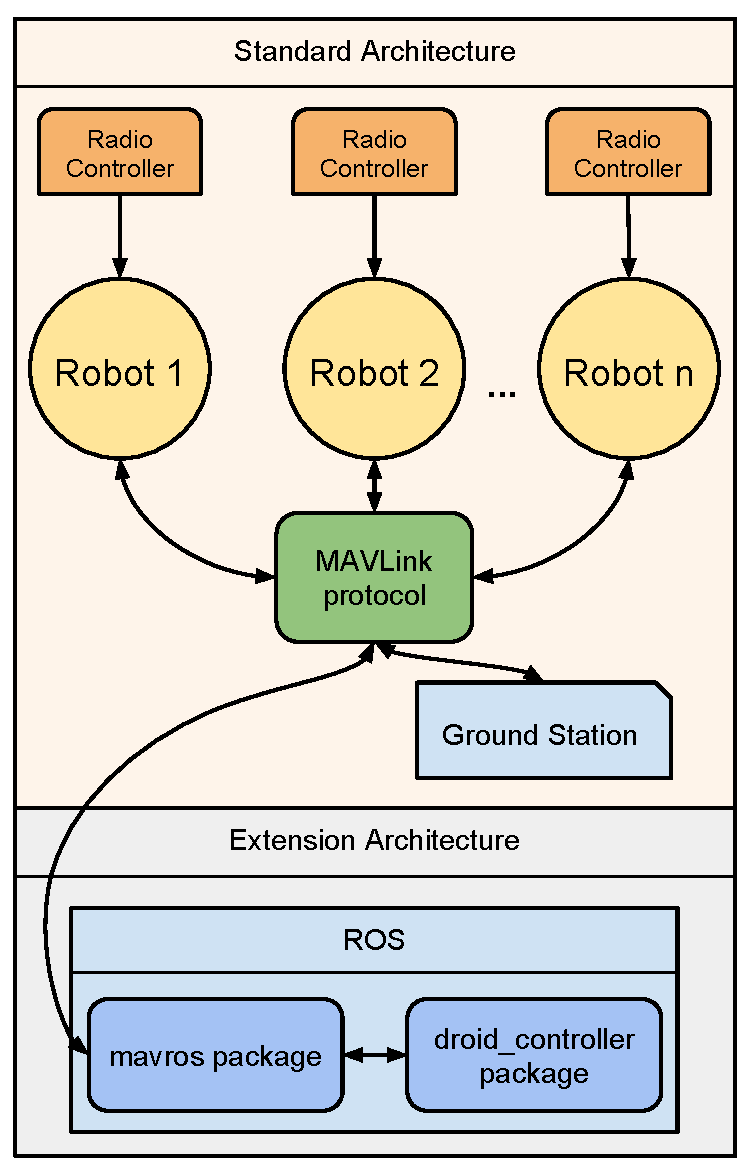
\includegraphics[width=0.8\columnwidth]{img/arquitetura.pdf}
  \caption{System Architecture}
  \label{fig:architecture}
\end{figure}

The MAVLink protocol is a standard regarding communication with autonomous systems, in this way there are several libraries that abstract the low-level details in communication, providing an interface for sending and receiving data transparently.
One of these libraries, implemented within the context of the ROS is the \emph{mavros} package.
This package continue in development by a group of nonprofit developers who created the tool because they see the opportunity of using these systems as autonomous intelligent agents.

The \emph{mavros} package is able to encode and decode messages in MAVLink, extract information and then format them into ROS messages, making the communication with a ArduPilot direct to the ROS infrastructure, providing easy access to other packages for these information.

Based on this structure, was created the package \emph{Droid Controller}, which contains a set of classes and algorithms that perform the reading of information from the agents and performs processing and exchange of information between them.

% subsection arquitetura (end)

\subsection{Droid Controller Package} % (fold)
\label{sub:droid_controller_package}

The \emph{Droid} package stacks over the \emph{mavros} package using it connection and MAVLink message handler.
The main goal was to create a set of classes that listen, store and share data from the agents and also create a interaction interface where is possible to request this data, send commands or missions.
This package should serve as basis for the creation of complex missions using the shared information between the robots.

The following are the main classes of the \emph{Droid} package:

\begin{description}
  \item[\textbf{Droid}] \hfill \\
    The Droid class is the base class to any specialized vehicle.
    It retains all important data about the robot like its current position, status of motors, MAVLink mode, current mission, battery status and others.
    Also export functions to get/set configuration parameters, send mission or arm the robot, among others.
  \item[\textbf{DroidCopter}] \hfill \\
    Specific class for a aerial robot, like a quadrotor.
    It uses and extends the Droid class, adding behaviors to return the craft to ground based on the level of remaining battery, and perform the initialization sequence for a mission.
  \item[\textbf{DroidRover}] \hfill \\
    Class that control a terrestrial robot, like a rover.
    Extends the Droid class to perceive for obstacles while a mission, requesting for another agent to continue the mission if it's not possible to complete it.
\end{description}

As a example of integration and exchange of information, the Droid class implements a follow behavior, where a agent is capable of maintain a certain distance from another based on its current global position and the position of another robot.
This behavior can be extended to create a squad behavior using various robots.

% subsection droid_controller_package (end)

\section{EXPERIMENTS}
\label{sec:experiments}

The created architecture was tested in two environments: a simulation and a real.
The real agents are as shown the figure \ref{fig:agents}.
The primary objective was to prove that the connection and exchange of information occurs between the agents, in such way that each agent know about the others and can perform actions based on this knowledge.

To proof the \emph{Droid} package, two simulation tests was performed: (i) the following mode, where a agent must follow and maintain a certain distance from another target agent, and (ii) the obstacle mode, where a terrestrial agent can ask for help to a aerial agent if it detects that is not possible to complete your mission.

\begin{figure}[ht!]
  \centering
  \begin{subfigure}[b]{0.8\columnwidth}
    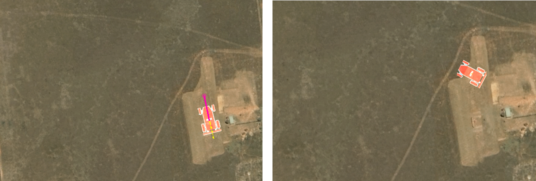
\includegraphics[width=\textwidth]{img/follow1.png}
  \end{subfigure}
  \begin{subfigure}[b]{0.8\columnwidth}
    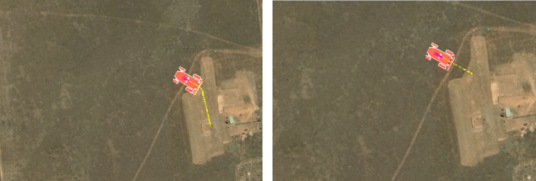
\includegraphics[width=\textwidth]{img/follow2.png}
  \end{subfigure}
  \begin{subfigure}[b]{0.8\columnwidth}
    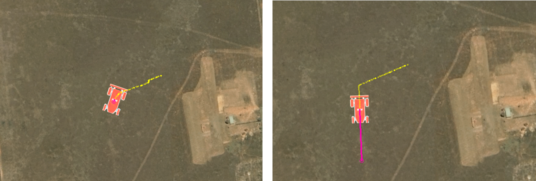
\includegraphics[width=\textwidth]{img/follow3.png}
  \end{subfigure}
  \begin{subfigure}[b]{0.8\columnwidth}
    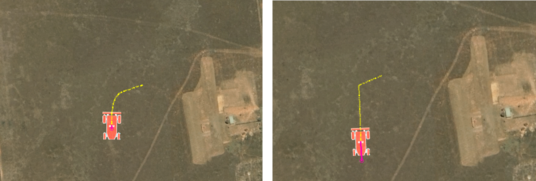
\includegraphics[width=\textwidth]{img/follow4.png}
  \end{subfigure}
  \begin{subfigure}[b]{0.8\columnwidth}
    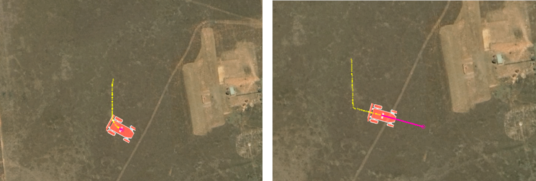
\includegraphics[width=\textwidth]{img/follow5.png}
  \end{subfigure}
  \begin{subfigure}[b]{0.8\columnwidth}
    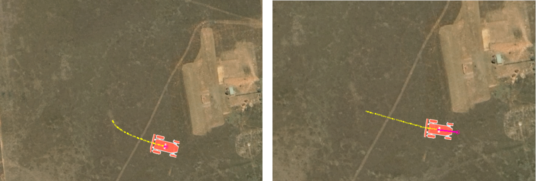
\includegraphics[width=\textwidth]{img/follow6.png}
  \end{subfigure}
  \begin{subfigure}[b]{0.8\columnwidth}
    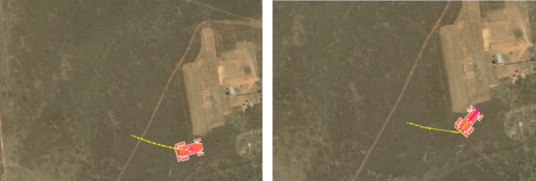
\includegraphics[width=\textwidth]{img/follow7.png}
  \end{subfigure}

  \caption{Two rovers in simulation, the right rover executes his mission while the left rover follows it.}
  \label{fig:simulation}
\end{figure}

\begin{figure*}
  \centering
  \begin{subfigure}[b]{0.9\columnwidth}
    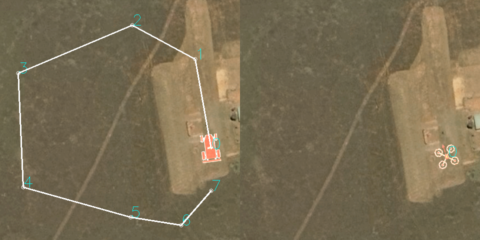
\includegraphics[width=\textwidth]{img/mission1.png}
    \caption{Mission start.}
  \end{subfigure}
  \begin{subfigure}[b]{0.9\columnwidth}
    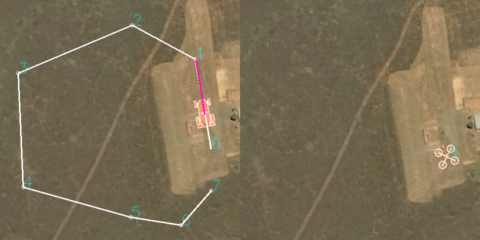
\includegraphics[width=\textwidth]{img/mission2.png}
    \caption{Go to waypoint 1.}
  \end{subfigure}
  \begin{subfigure}[b]{0.9\columnwidth}
    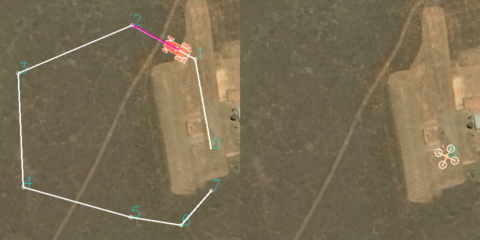
\includegraphics[width=\textwidth]{img/mission3.png}
    \caption{Go to waypoint 2.}
  \end{subfigure}
  \begin{subfigure}[b]{0.9\columnwidth}
    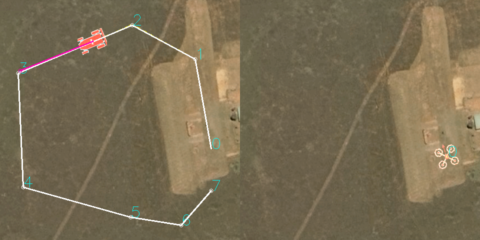
\includegraphics[width=\textwidth]{img/mission4.png}
    \caption{Go to waypoint 3.}
  \end{subfigure}
  \begin{subfigure}[b]{0.9\columnwidth}
    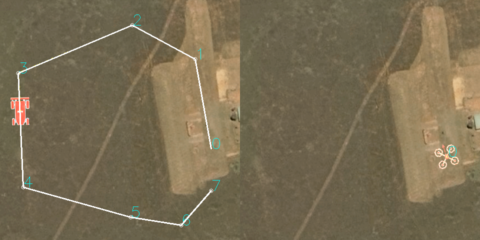
\includegraphics[width=\textwidth]{img/mission5.png}
    \caption{Go to waypoint 4, but found a obstacle.}
  \end{subfigure}
  \begin{subfigure}[b]{0.9\columnwidth}
    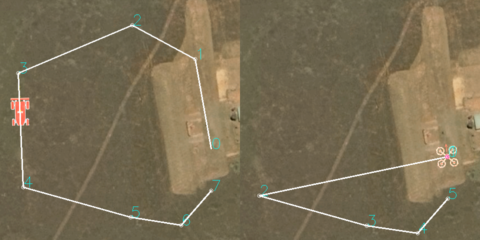
\includegraphics[width=\textwidth]{img/mission6.png}
    \caption{Request help and send the remainder mission.}
  \end{subfigure}
  \begin{subfigure}[b]{0.9\columnwidth}
    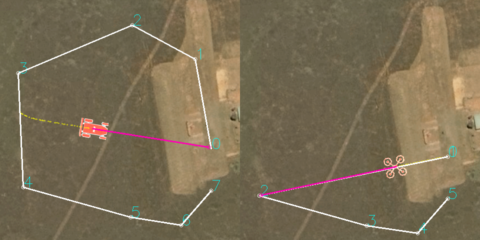
\includegraphics[width=\textwidth]{img/mission7.png}
    \caption{Return to home while other agent take the mission.}
  \end{subfigure}
  \begin{subfigure}[b]{0.9\columnwidth}
    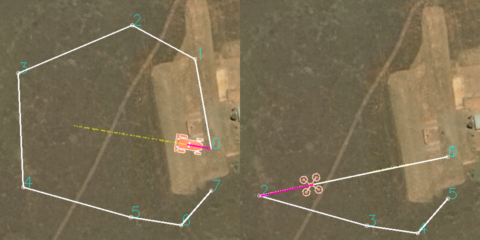
\includegraphics[width=\textwidth]{img/mission8.png}
    \caption{Reach home and the helper agent start the mission.}
  \end{subfigure}
  \begin{subfigure}[b]{0.9\columnwidth}
    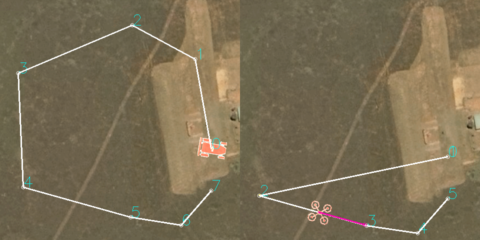
\includegraphics[width=\textwidth]{img/mission9.png}
    \caption{The agent continue the mission.}
  \end{subfigure}
  \begin{subfigure}[b]{0.9\columnwidth}
    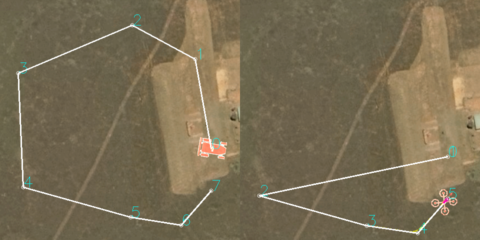
\includegraphics[width=\textwidth]{img/mission10.png}
    \caption{Mission complete by the other agent.}
  \end{subfigure}

  \caption{Mission execution by the rover agent, that founds a obstacles and ask for help to another agent.}
  \label{fig:simulation_mission}
\end{figure*}

The following mode test is demonstrated in the figure \ref{fig:simulation} (simulation environment) and \ref{fig:real} (real experiment), where one robot is executing a determined mission, but sharing its current position the other agents in the team, and another robot use this information to follow that agent, but keeping a configurable safety distance.

% The figure \ref{fig:simulation} show the two agents in the simulation representation.
% They have similar capabilities compared to the real robots, but with a best control and maneuverability, considering that a simulation will not is equal to a real environment.

\begin{figure}[ht!]
  \centering
  \begin{subfigure}[b]{0.8\columnwidth}
    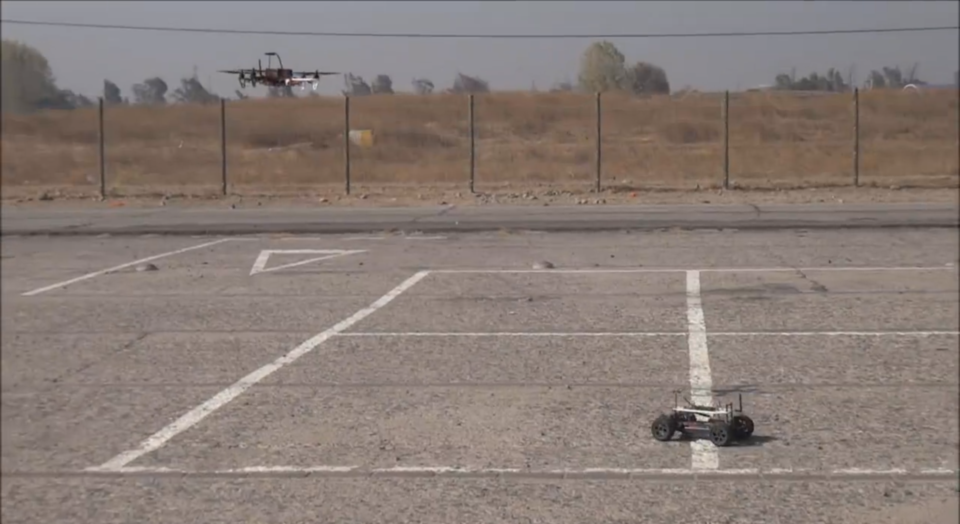
\includegraphics[width=\textwidth]{img/follow_real1.png}
  \end{subfigure}
  \begin{subfigure}[b]{0.8\columnwidth}
    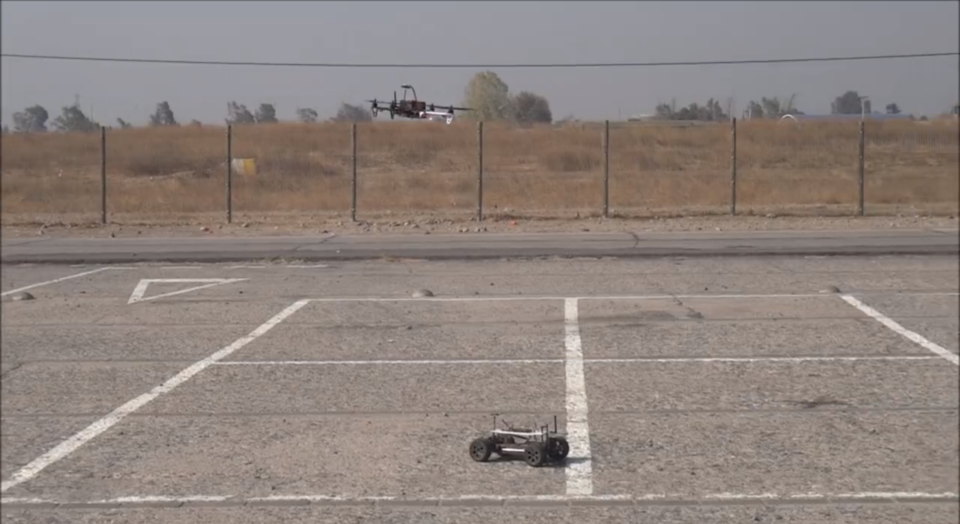
\includegraphics[width=\textwidth]{img/follow_real2.png}
  \end{subfigure}
  \begin{subfigure}[b]{0.8\columnwidth}
    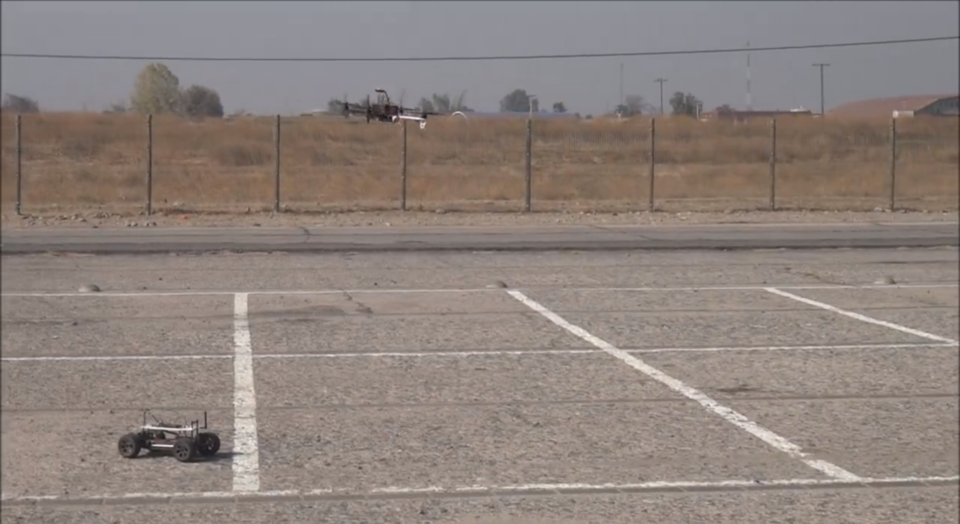
\includegraphics[width=\textwidth]{img/follow_real3.png}
  \end{subfigure}
  \begin{subfigure}[b]{0.8\columnwidth}
    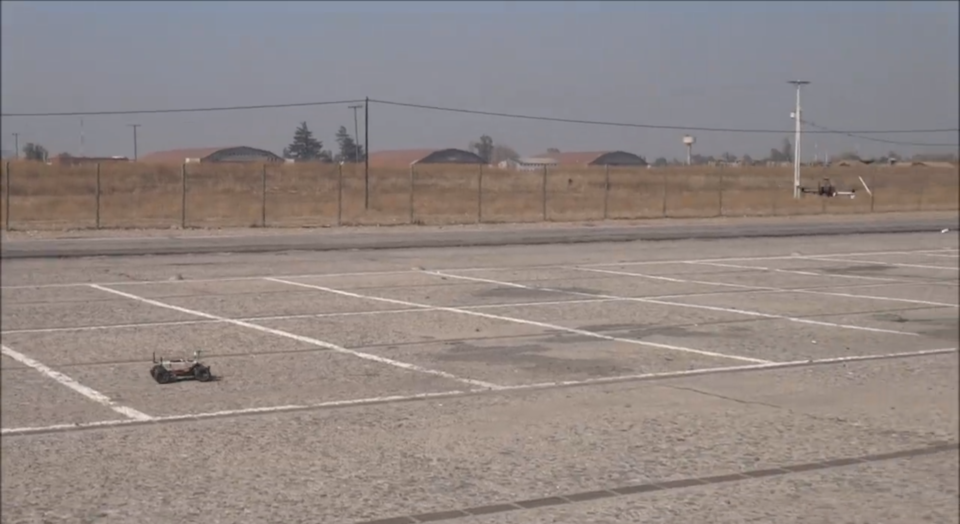
\includegraphics[width=\textwidth]{img/follow_real4.png}
  \end{subfigure}

  \caption{Real experiment showing the follow mode using a rover vehicle and a quadrotor drone.}
  \label{fig:real}
\end{figure}

The test shown in the figure \ref{fig:simulation_mission} demonstrate the behavior where a agent founds a obstacle which prevents your mission conclusion, and then ask to another agent to finish it, sending the remaining mission and returning the home.

These tests were developed to demonstrate that the architecture extension works to communicate and take decisions based on data sent by the agents, performing actions using the resources available for the team of robots.

% The first test applied was to just make one agent follow another while

\section{CONCLUSIONS AND FUTURE WORK}
\label{sec:conclusion}

In this work was presented a extension of the standard architecture of control of a autonomous agent using the ArduPilot autopilot controller communicating using the MAVLink protocol that guarantees communication and information exchange between a team of robots.
The experiments showed the capabilities of the extension, using the available data to take control of the agents.

Future directions include the addition of a squad control, where multiple agents can perform missions of surveillance or search, exchanging data about the supervised area among then and with a land base.
Another improvement is to add support for other types of robots and uses the individual abilities to improve the team.


\section{Acknowledgment} % (fold)
\label{sec:acknowledgment}

I would like to thank the opportunity to have participated in research at the University of Santiago de Chile, to teachers Arturo Alvarez Cea and Gonzalo Acuna, by the knowledge exchange, and SISAR Ltda (www.sisar.cl) for providing the robots used during the experiments.
They were moments of learning and exchange of knowledge that have been and will be shared by both sides in future research to come.

% section acknowledgment (end)

\bibliographystyle{IEEEtran}
\bibliography{bibliography}

\end{document}
